\documentclass{standalone}
\usepackage{tikz}
\usepackage{ctex,siunitx}
\usepackage{tkz-euclide}
\usepackage{amsmath}
\usetikzlibrary{patterns, calc}
\usetikzlibrary {decorations.pathmorphing, decorations.pathreplacing, decorations.shapes,}
\begin{document}
\small
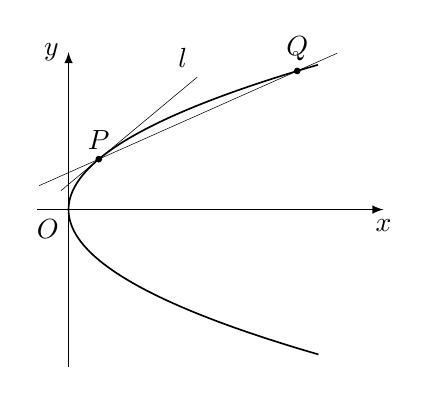
\begin{tikzpicture}[>=latex,scale=0.8]
  \draw[thin,->](-0.5,0)--(5,0)node[below]{$x$};
  \draw[thin,->](0,-2.5)--(0,2.5)node[left]{$y$};
  \tkzDefPoints{0/0/O,0.48/0.8/P,3.63/2.2/Q,1.68/1.8/Pl}
  \draw[semithick,domain=-2.3:2.3,samples=200] plot({0.75*\x*\x},{\x});
  % \draw[semithick](40,30)--(40,-30);
  \tkzDrawPoints[fill=black](P,Q)
  \tkzDrawLine[add = 0.3 and 0.2](P,Q)
  \tkzDrawLine[add = 0.5 and 0.3](P,Pl)
  \tkzLabelLine[pos=1.3,above left](P,Pl){$l$}
  \tkzLabelPoints[below left](O)
  \tkzLabelPoints[above](P,Q)
\end{tikzpicture}
\end{document}